\input templates/header

\usepackage{epigraph}
\usepackage[normalem]{ulem}
\usepackage{xcolor}
\usepackage{colortbl}
\usepackage{tikz}
\usepackage[normalem]{ulem}
\usepackage[absolute,overlay]{textpos}
\usetikzlibrary{trees}
\usetikzlibrary{shapes}
\usetikzlibrary{positioning}

\setlength{\epigraphwidth}{6cm}

\usepackage{xmpmulti}
\usepackage{listings}

\lstset{
  basicstyle=\ttfamily,
%  columns=fullflexible,
  keywordstyle=\color{red}\bfseries,
  commentstyle=\color{blue},
  showstringspaces=false,
  escapeinside={<@}{@>},
}

\newcommand*\circled[1]{\tikz[baseline=(char.base)]{
      \node[circle,ball color=blue, shade, 
 color=white,inner sep=1.2pt] (char) {\tiny #1};}}


\title[ASD - Programmazione Dinamica]{\textbf{Algoritmi e Strutture Dati}\\[24pt]Programmazione dinamica -- Parte 1}

\graphicspath{{figs/13/}}

\begin{document}



%-------------------------------------------------------------------------
\FrameTitle{}

%-------------------------------------------------------------------------
\FrameContent


%%%%%%%%%%%%%%%%%%%%%%%%%%%%%%%%%%%%%%%%%%%%%%%%%%%%%%%%%%%%%%%%%%%%%%%%%%
\section{Introduzione}
%%%%%%%%%%%%%%%%%%%%%%%%%%%%%%%%%%%%%%%%%%%%%%%%%%%%%%%%%%%%%%%%%%%%%%%%%%

\begin{frame}{Tecniche di soluzione problemi}

\BIL
\item Divide-et-impera 
\item Programmazione dinamica / memoization
\item Tecnica greedy
\item Ricerca locale 
\item Backtrack
\item Algoritmi probabilistici
\item Tecniche di soluzione per problemi intrattabili
\EIL

\end{frame}

\begin{frame}{Programmazione dinamica in pillole}

\BIL
\item Un metodo per spezzare un problema ricorsivamente in sottoproblemi
\item Ogni sottoproblema viene risolto una volta sola
\item La sua soluzione viene memorizzata in una tabella
\item Nel caso un sottoproblema debba essere risolto nuovamente, si ottiene la
  sua soluzione dalla tabella
\item La tabella è facilmente indirizzabile (lookup in $O(1)$)
\EIL
    
\epigraph{\alert{Those who cannot remember the past are condemned to repeat it}
}{\textit{George Santayana, 1905}}

\end{frame}




\begin{frame}{Approccio generale}

\vspace{-9pt}
\IGH{0.77}{progrdyn.pdf}

\end{frame}

\begin{frame}{Un po' di storia}

\begin{overprint}
\onslide<1|handout:1>
\BIL
\item Il termine \alert{Dynamic Programming} è stato coniato da Richard Bellman 
agli inizi degli anni '50, nell'ambito dell'ottimizzazione matematica   
\item Inizialmente, si riferiva al processo di risolvere un problema compiendo
le migliori decisioni una dopo l'altra.
\item "Dynamic" doveva dare un senso "temporale"
\item "Programming" si riferiva all'idea di creare "programmazioni ottime",
per esempio nel campo della logistica
\EIL

\bigskip
\url{https://en.wikipedia.org/wiki/Dynamic_programming\#History}
\onslide<2|handout:0>
\IGH{0.8}{dynamic-entropy.png}
\vspace{-12pt}
\small
\url{https://xkcd.com/2318/}
\end{overprint}
\end{frame}



%%%%%%%%%%%%%%%%%%%%%%%%%%%%%%%%%%%%%%%%%%%%%%%%%%%%%%%%%%%%%%%%%%%%%%%%%%
\section{Domino}
%%%%%%%%%%%%%%%%%%%%%%%%%%%%%%%%%%%%%%%%%%%%%%%%%%%%%%%%%%%%%%%%%%%%%%%%%%

\begin{frame}{Problema 1 -- Domino lineare}

\vspace{-9pt}
\begin{myboxtitle}[Definizione]
Il gioco del domino è basato su tessere di dimensione $2 \times 1$. Scrivere
un algoritmo efficiente che prenda in input un intero $n$ e restituisca il numero di possibili disposizioni di $n$ tessere in un rettangolo $2 \times n$.
\end{myboxtitle}

\begin{myboxtitle}[Esempio]
I casi (a)-(e) della figura rappresentano le cinque disposizioni possibili con cui è possibile riempire un rettangolo $2 \times 4$. 
\end{myboxtitle}

\begin{center}
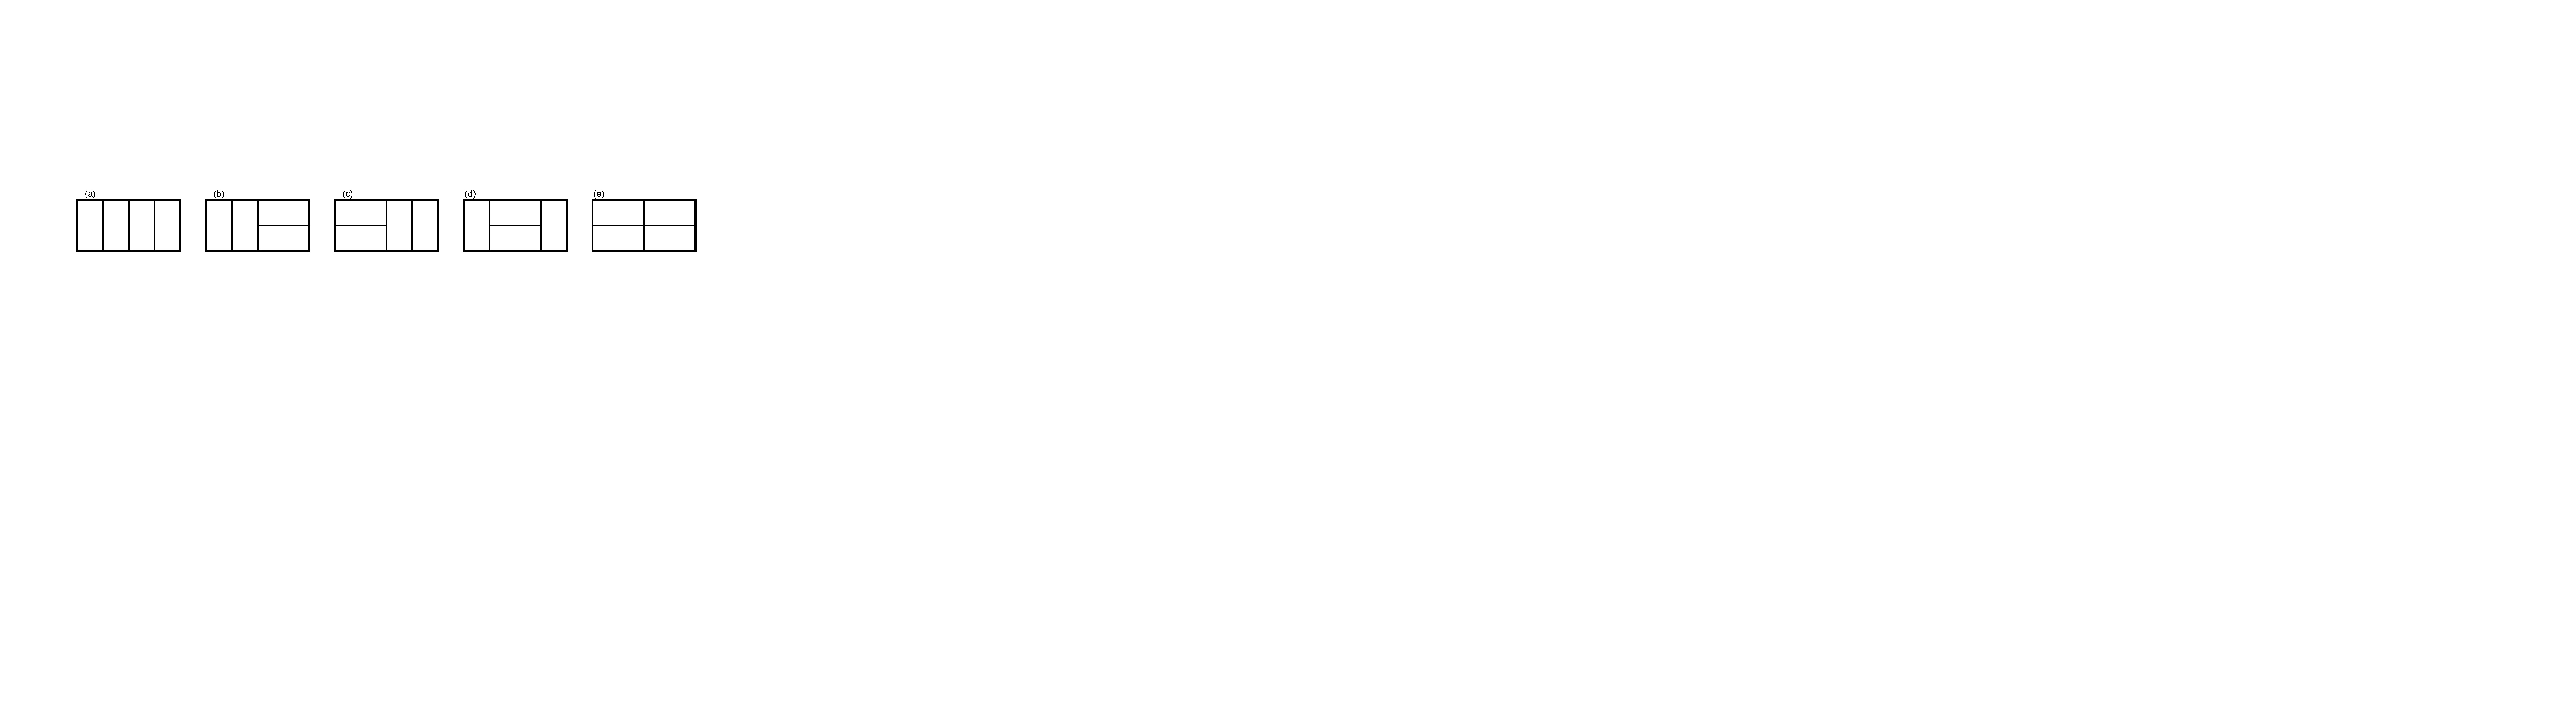
\includegraphics[width=1.0\textwidth]{domino.pdf}
\end{center}

\end{frame}


%-------------------------------------------------------------------------
\begin{frame}[fragile]{Domino}

\vspace{-9pt}
\BB{Quante disposizioni ci sono per $n=7$?}

\begin{center}
\begin{tabular}{m{7cm}m{3cm}}
Wooclap.com, codice: \href{https://app.wooclap.com/ZAEBFA}{\alert{\underline{ZAEBFA}}}
&

\includegraphics[width=1.8cm]{qrcode-13-pd1.png}\\
\end{tabular}
\end{center}

\bigskip
Hint: calcola quante disposizioni ci sono per $n=0 \ldots 7$ 

\bigskip
\BB{Come risolvereste il problema?}


\end{frame}

%-------------------------------------------------------------------------
\begin{frame}{Domino}

\vspace{-9pt}
\begin{myboxtitle}[Definizione ricorrenza]
Definiamo una formula ricorsiva $\mathit{DP}[n]$ che permetta di calcolare il numero di disposizioni possibili quando si hanno $n$ tessere.
\end{myboxtitle}

\begin{overprint}
\onslide<1|handout:0>
\BIL
\item Quante disposizioni possibili se non ho tessere ($n=0$)?
\item Quante disposizioni possibili se ho solo una tessera ($n=1$)?
\EIL
\onslide<2|handout:1>
\BIL
\item Con $n=0$, esiste una sola disposizione possibile (nessuna tessera)
\item Con $n=1$, esiste una sola disposizione possibile (tessera verticale)
\EIL
\onslide<3|handout:0>
\BIL
\item Cosa succede se decido di mettere l'ultima tessera in verticale?
\item Cosa succede se decido di mettere l'ultima tessera in orizzontale?
\EI
\onslide<4|handout:2>
\BIL
\item Se metto una tessera in verticale, risolverò il problema
di dimensione $n-1$
\item Se metto una tessera in orizzontale, ne devo mettere due; risolverò
il problema di dimensione $n-2$
\item Queste due possibilità si sommano insieme (conteggio)
\EIL
\end{overprint}

\bigskip
\begin{overprint}
\onslide<1|handout:0>
\[
\mathit{DP}[n] = \begin{cases}
  ? & n \leq 1 \\
  \makebox[3.5cm][l]{?} & n>1
\end{cases}
\]
\onslide<2-3|handout:1>
\[
\mathit{DP}[n] = \begin{cases}
  1 & n \leq 1 \\
  \makebox[3.5cm][l]{?} & n>1
\end{cases}
\]
\onslide<4|handout:2>
\[
\mathit{DP}[n] = \begin{cases}
  1 & n \leq 1 \\
  \mathit{DP}[n-2]+\mathit{DP}[n-1] & n>1
\end{cases}
\]
\end{overprint}

\end{frame}

\begin{frame}<1|handout:0>[fragile]{Serie matematica}

\vspace{-9pt}
\BB{La serie generata è la seguente}

\begin{lstlisting}
1, 1, 2, 3, 5, 8, 13, 21, 34, 55, 89, ...
\end{lstlisting}

\BB{Ricorda niente?}

\end{frame}


\begin{frame}[fragile]{Serie matematica}

\vspace{-9pt}
\BB{La serie generata è la seguente}

\begin{lstlisting}
1, 1, 2, 3, 5, 8, 13, 
21, 34, 55, 89, ...
\end{lstlisting}

\begin{textblock*}{5cm}(7.6cm,0.6cm) % {block width} (coords)
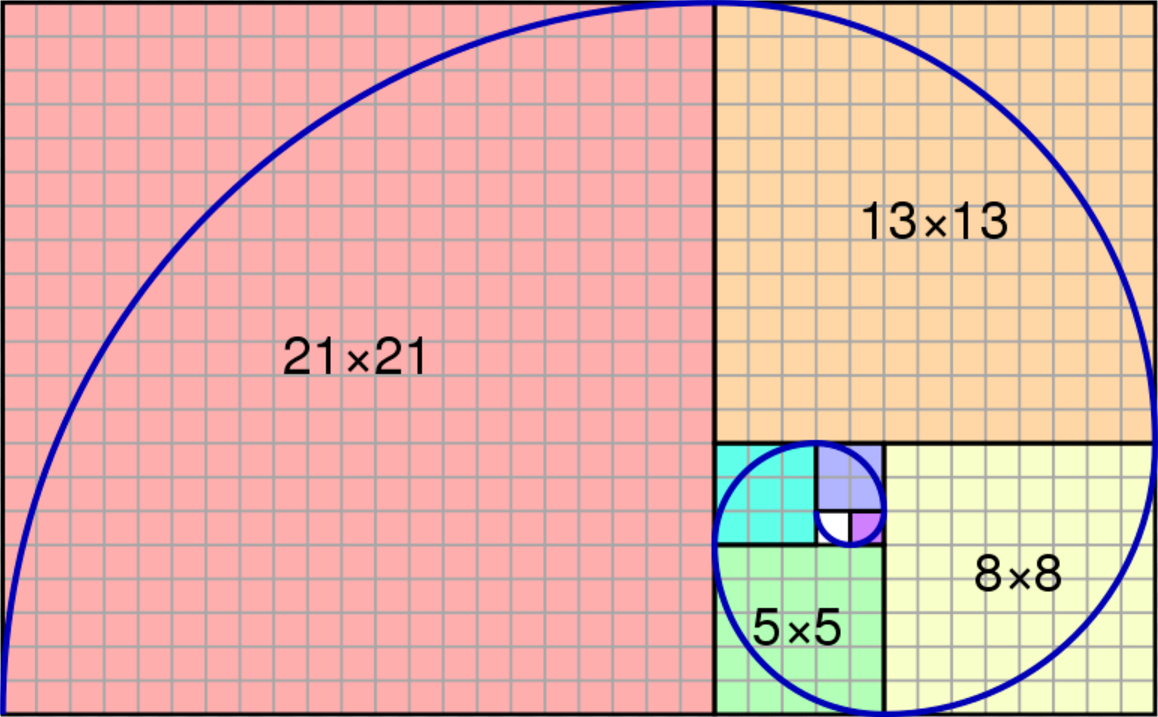
\includegraphics[width=5cm]{fibonacci.png}
\end{textblock*}

\begin{myboxtitle}[Successione di Fibonacci]
$\mathit{DP}[n]$ è pari al $(n+1)$-esimo numero della serie di Fibonacci, introdotta da Leonardo Pisano detto il Fi'Bonacci (1175--1235).
\end{myboxtitle}

\BIL
\item Definiti per descrivere la crescita di una popolazione di conigli (!)
\item In natura: Pigne, conchiglie, parte centrale dei girasoli, etc.
\item In informatica: Alberi AVL minimi, Heap di Fibonacci, etc.
\EIL

\end{frame}


\begin{frame}[fragile]{Domino - Algoritmo ricorsivo}

\vspace{-9pt}
\BB{Algoritmo ricorsivo che risolve il problema Domino}
\begin{Procedure}
\caption[A]{\INTEGER\ \textsf{domino1}(\INTEGER\ $n$)}
  \eIf{$n \leq 1$}{
    \Return $1$\;
  }{
    \Return $\textsf{domino1}(n-1) + \textsf{domino1}(n-2)$\;
  }
\end{Procedure}

\BB{Qual è l'equazione di ricorrenza associata a \textsf{domino1()}?}
\begin{center}
\begin{tabular}{m{7cm}m{3cm}}
Wooclap.com, codice: \href{https://app.wooclap.com/ZAEBFA}{\alert{\underline{ZAEBFA}}}
&

\includegraphics[width=1.8cm]{qrcode-13-pd1.png}\\
\end{tabular}
\end{center}


\end{frame}

\begin{frame}{Complessità computazionale}

\vspace{-9pt}
\BB{Equazione di ricorrenza associata a \textsf{domino1()}}

\[
  T(n) = \begin{cases}
  1 & n \leq 1 \\
  T(n-1)+T(n-2)+1 & n > 1\\
  \end{cases}
\]

\BB{Qual è la complessità di \textsf{domino1()}?}
\pause
Ricorrenza lineare di ordine costante:
\BI
\item $a_1 = 1, a_2=1, a= a_1+a_2 = 2, \beta=0$
\item Complessità: $\Theta(a^n \cdot n^\beta)$
\EI

\[
T(n) = \Theta(2^n)
\]

\end{frame}

%-------------------------------------------------------------------------
\begin{frame}{Albero di ricorsione di \textsf{domino1()}}
  
\IG{0.9}{fibonacci-tree.pdf}

\vspace{-12pt}
\begin{flushright}
Molti sotto-problemi ripetuti!
\end{flushright}
\end{frame}

%-------------------------------------------------------------------------
\begin{frame}{Come evitare di risolvere un problema più di una volta}
  
\vspace{-9pt}
\begin{myboxtitle}[Tabella DP]
\BIL
\item Memorizziamo il risultato ottenuto risolvendo un particolare problema
in una \alert{tabella $\mathit{DP}$} (vettore, matrice, dizionario)
\item La tabella deve contenere un elemento per ogni sottoproblema che dobbiamo risolvere
\EIL
\end{myboxtitle}

\begin{myboxtitle}[Casi base]
\BIL
\item Memorizziamo i casi base direttamente nelle posizioni relative
\EIL
\end{myboxtitle}

\begin{myboxtitle}[Iterazione bottom-up]
\BIL
\item Si parte dai problemi risolubili come basi base
\item Si sale verso problemi via via più grandi ...
\item ... fino a raggiungere il problema originale
\EIL
\end{myboxtitle}

\end{frame}



%-------------------------------------------------------------------------
\begin{frame}[fragile]{Domino: algoritmo iterativo}

\vspace{-9pt}
\BB{Algoritmo iterativo che risolve il problema Domino}

\begin{Procedure}
\caption[A]{\INTEGER\ \textsf{domino2}(\INTEGER $n$)}
  $\mathit{DP} = \NEW\ \INTEGER[0 \ldots n]$\;
  $\mathit{DP}[0] = \mathit{DP}[1] = 1$\;
  \For{$i = 2$ \TO\ $n$}{
    $\mathit{DP}[i] = \mathit{DP}[i-1] + \mathit{DP}[i-2]$\;
  }
  \Return $\mathit{DP}[n]$\;
\end{Procedure}

\begin{center}
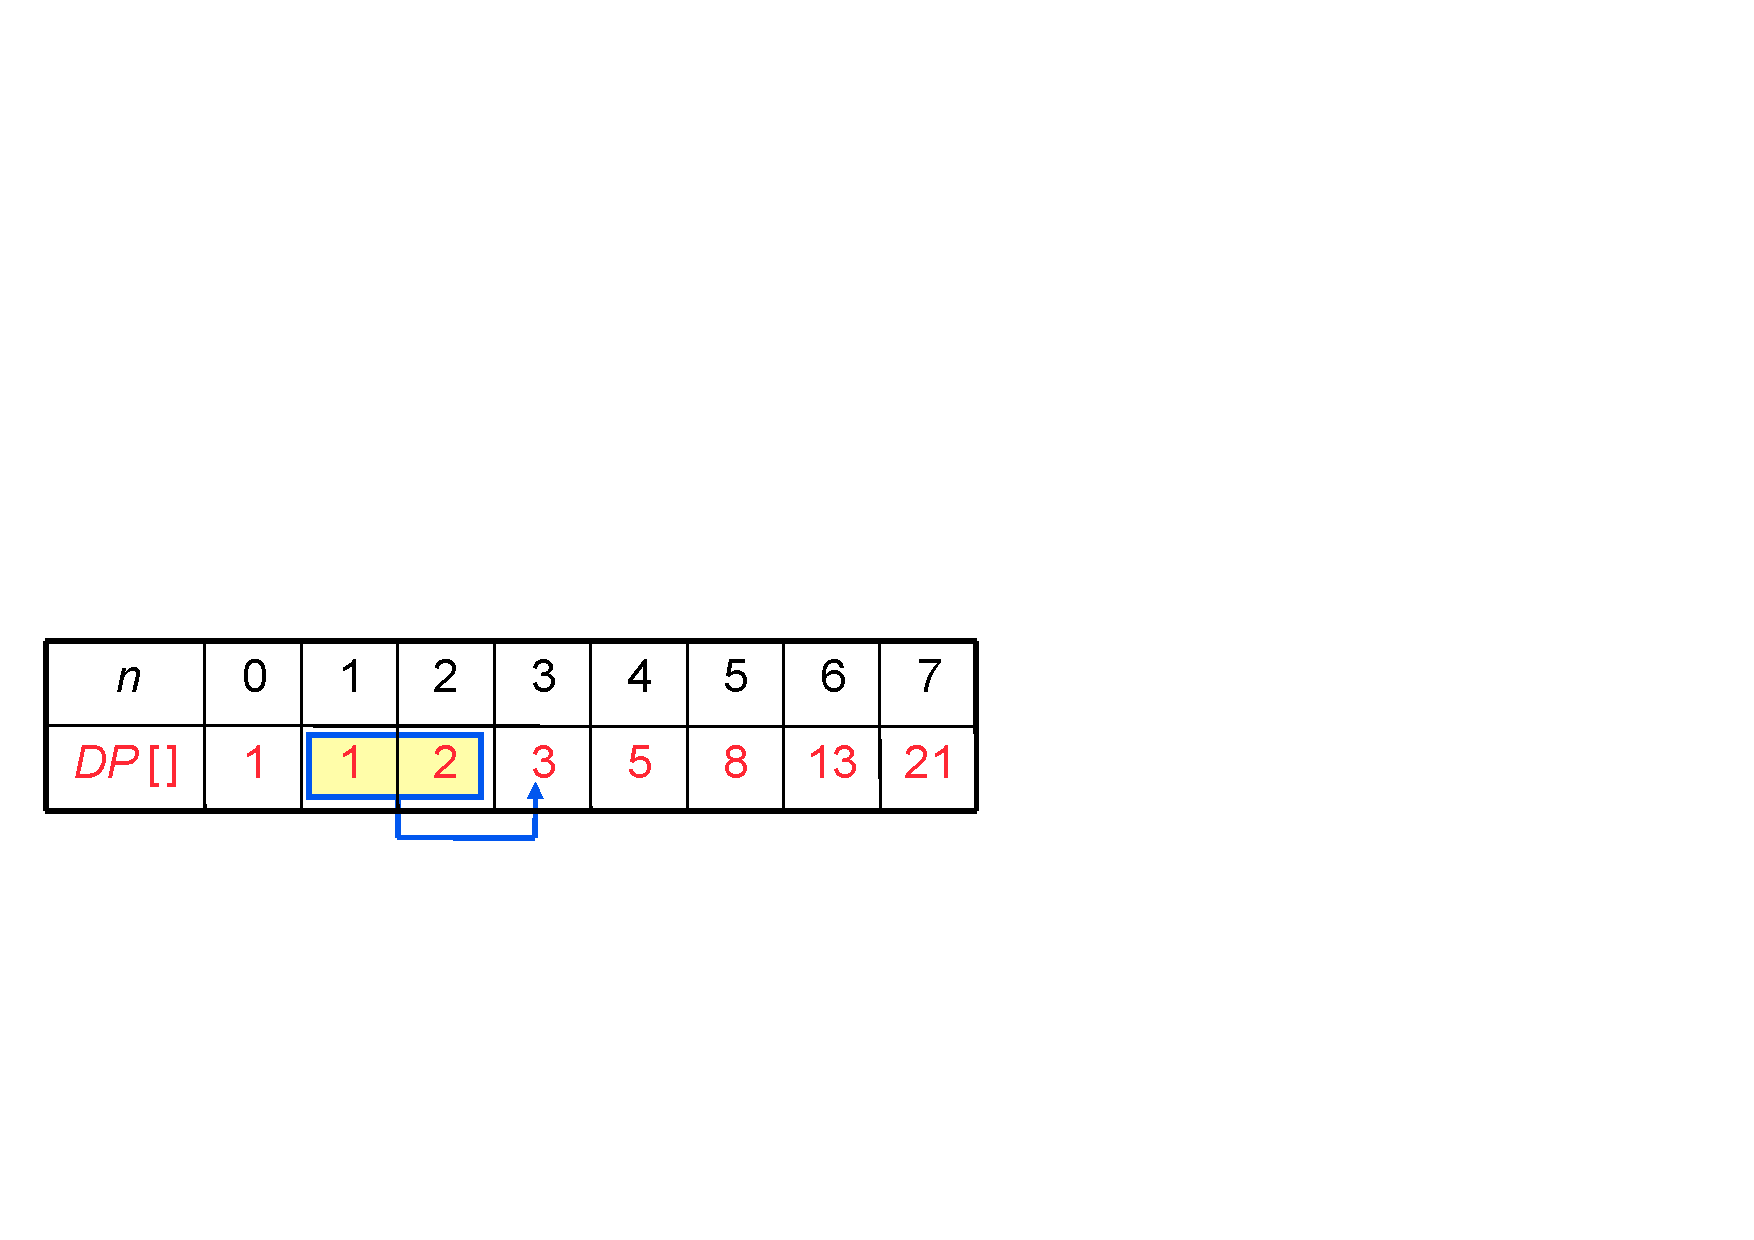
\includegraphics[width=0.75\textwidth]{fib-table1.pdf}
\end{center}

\end{frame}



%-------------------------------------------------------------------------
\begin{frame}[fragile]{Domino}

\vspace{-9pt}
\begin{Procedure}
\caption[A]{\INTEGER\  \textsf{domino2}(\INTEGER $n$)}
  $\mathit{DP} = \NEW\ \INTEGER[0 \ldots n]$\;
  $\mathit{DP}[0] = \mathit{DP}[1] = 1$\;
  \For{$i = 2$ \TO\ $n$}{
    $\mathit{DP}[i] = \mathit{DP}[i-1] + \mathit{DP}[i-2]$\;
  }
  \Return $\mathit{DP}[n]$\;
\end{Procedure}

\begin{columns}[T]
\column{0.72\textwidth}
\BB{Qual è la complessità in \alert{tempo} di $\textsf{domino2}(n)$?}
\pause
\column{0.27\textwidth}
\bigskip
\alert{$T(n) = \Theta(n)$}
\end{columns}

\begin{columns}[T]
\column{0.72\textwidth}
\BB{Qual è la complessità in \alert{spazio} di $\textsf{domino2}(n)$?}
\pause
\column{0.27\textwidth}
\bigskip
\alert{$S(n) = \Theta(n)$}
\end{columns}

\begin{columns}[T]
\column{0.72\textwidth}
\BB{Possiamo fare \alert{"meglio di così"}?}
\pause
\column{0.27\textwidth}
\bigskip
\alert{Possiamo ridurre lo spazio utilizzato}
\end{columns}

\end{frame}

%-------------------------------------------------------------------------
\begin{frame}[fragile]{Domino}

\vspace{-9pt}
	\begin{columns}[T]
\column{0.38\textwidth}
\vspace{-8pt}
\begin{Procedure}
\caption[A]{\INTEGER\ \textsf{domino3}(\INTEGER\ $n$)}
  $\INTEGER\ \mathit{DP_0} = 1$\;
  $\INTEGER\ \mathit{DP_1} = 1$\;
  $\INTEGER\ \mathit{DP_2} = 1$\;
  \For{$i = 2$ \TO\ $n$}{
    $\mathit{DP_0} = \mathit{DP_1}$\;
    $\mathit{DP_1} = \mathit{DP_2}$\;
    $\mathit{DP_2} = \mathit{DP_0} + \mathit{DP_1}$\;
  }
  \Return $\mathit{DP}_2$\;
\end{Procedure}
\column{0.62\textwidth}

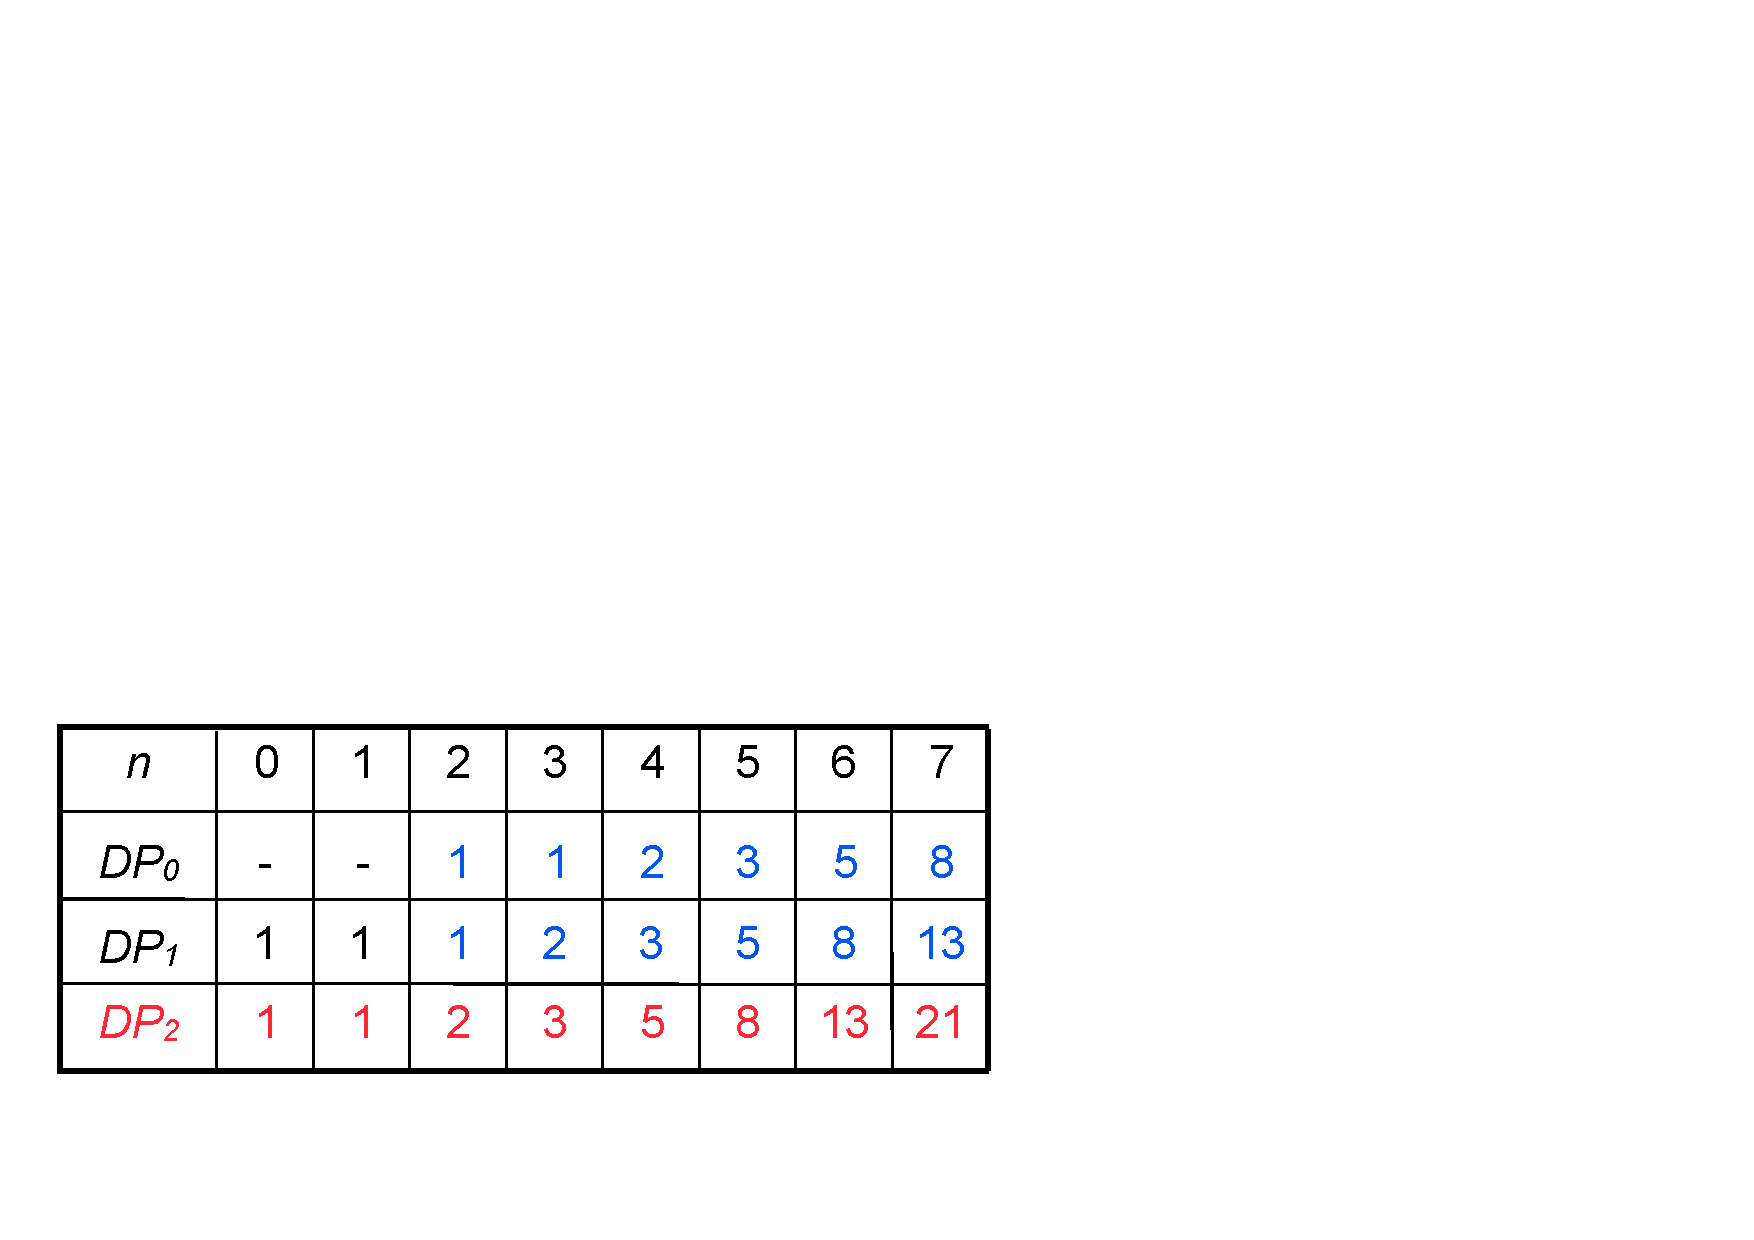
\includegraphics[width=\textwidth]{fib-table2.pdf}

\end{columns}

\begin{columns}[T]
\column{0.72\textwidth}
\BB{Qual è la complessità in \alert{spazio} di $\textsf{domino3}(n)$?}
\pause
\column{0.28\textwidth}
\bigskip
\alert{$S(n) = \Theta(1)$}
\end{columns}

\end{frame}



\begin{frame}[fragile]{Ripasso sulla complessità computazionale}

\vspace{-9pt}
\BB{Siete sicuri che i calcoli sulla complessità siano corretti?}

\pause
\bigskip
\BB{Osservate di nuovo la serie generata}

\begin{lstlisting}
1, 1, 2, 3, 5, 8, 13, 21, 34, 55, 89, 144, ...
\end{lstlisting}

\bigskip
\BB{Quanti bit sono necessari per memorizzare $F(n)$?}

\end{frame}


\begin{frame}{Modello costo uniforme vs modello costo logaritmico}

\vspace{-9pt}
\begin{myboxtitle}[Formula di Binet per i numeri di Fibonacci]
\vspace{6pt}
\begin{columns}[T]
\column{0.75\textwidth}
\[
\mathit{DP}[n-1] = F(n) = \frac{\phi^n}{\sqrt{5}} - \frac{(1-\phi)^n}{\sqrt{5}} 
\]
dove $\phi$ è la \alert{sezione aurea}:
\begin{align*}
\phi &={1+\sqrt 5 \over 2}=1{,}6180339887\dots  \\
\frac{1}{\phi} = \phi - 1 & ={2 \over 1+\sqrt 5 }=0{,}6180339887\dots 
\end{align*}
\column{0.20\textwidth}
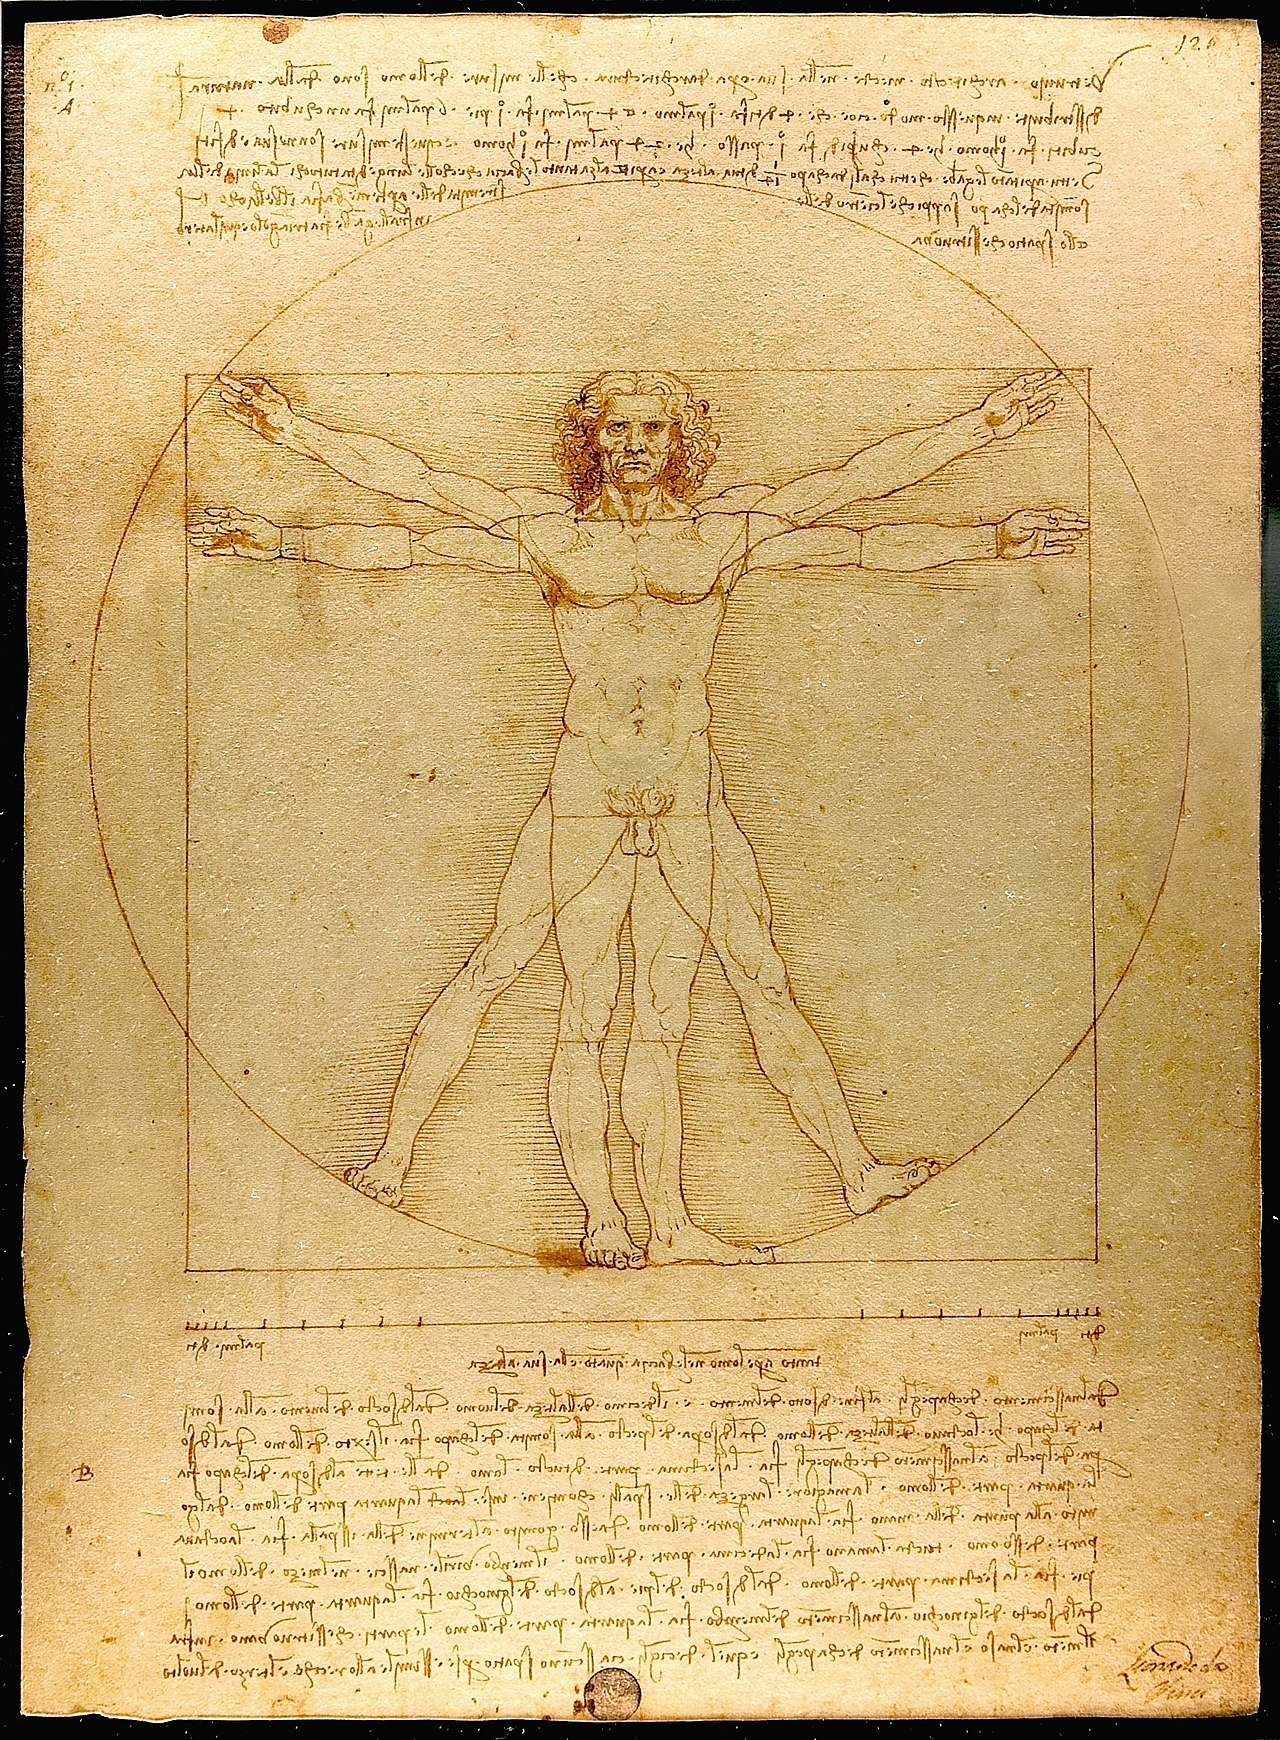
\includegraphics[width=\textwidth]{vitruviano.jpg}
\end{columns}
\end{myboxtitle}


\begin{columns}[T]
\column{0.75\textwidth}
\vspace{-6pt}
\BB{Quanti bit sono richiesti per memorizzare $F(n)$?}
\BB{Quanto costa sommare due numeri di Fibonacci consecutivi?}
\pause
\column{0.25\textwidth}

\bigskip
\bigskip
\alert{$\log F(n) = \Theta(n)$}
\end{columns}

\end{frame}


\begin{frame}{Modello costo uniforme vs modello costo logaritmico}
  
Nel modello di costo logaritmico, le tre versioni hanno complessità:

\begin{center}
\begin{tabular}{|c|c|c|}
\hline
\textbf{Funzione} & \textbf{Complessità (Tempo)} & \textbf{Complessità (Spazio)} \\\hline
\textsf{domino1()} & $O(n2^n)$ & $O(n^2)$ \\\hline
\textsf{domino2()} & $O(n^2)$ & $O(n^2)$ \\\hline
\textsf{domino3()} & $O(n^2)$ & $O(n)$ \\\hline
\end{tabular}
\end{center}

\bigskip
Se siete curiosi, si può risolvere il problema in tempo $O(n \log n)$ utilizzando l'esponenziazione di matrici basata su quadrati o un algoritmo che sfrutta una proprietà dei numeri di Fibonacci:

\bigskip
\url{https://jeffe.cs.illinois.edu/teaching/algorithms/book/03-dynprog.pdf}


\end{frame}

%%%%%%%%%%%%%%%%%%%%%%%%%%%%%%%%%%%%%%%%%%%%%%%%%%%%%%%%%%%%%%%%%%%%%%%%%%%%%
\section{Hateville}
%%%%%%%%%%%%%%%%%%%%%%%%%%%%%%%%%%%%%%%%%%%%%%%%%%%%%%%%%%%%%%%%%%%%%%%%%%%%%

\begin{frame}{Hateville}

\BIL
\item Hateville è un villaggio particolare, composto da $n$ case, numerate da $1$ a 
$n$ lungo una singola strada. 

\item Ad Hateville ognuno odia i propri vicini della 
porta accanto, da entrambi i lati.
\item Quindi, il vicino $i$ odia i vicini $i-1$ e $i+1$ (se esistenti). 

\item Hateville vuole organizzare una sagra e vi 
ha affidato il compito di raccogliere i fondi. 

\item Ogni abitante $i$ ha intenzione
di  donare una quantità $D[i]$, ma non intende partecipare ad una raccolta 
fondi a cui partecipano uno o entrambi i propri vicini. 

\EIL

\end{frame}

\begin{frame}{Hateville}

\vspace{-9pt}
\begin{myboxtitle}[Problemi]
\BIL
\item Scrivere un algoritmo che dato il vettore $D$, restituisca la quantità massima di
fondi che può essere raccolta
\item Bonus: restituire un sottoinsieme di indici 
$S \subseteq \{ 1, \ldots, n \}$ tale che il totale dei fondi raccolti
$T = \sum_{i \in S} D[i]$ sia massimale
\EIL
\end{myboxtitle}

\begin{myboxtitle}[Qual è la donazione massima con \alert{$D = [4, 3, 6, 5, 8, 7]$?}]
\vspace{-6pt}
\begin{tabular}{m{7cm}m{3cm}}
Wooclap.com, codice: \href{https://app.wooclap.com/ZAEBFA}{\alert{\underline{ZAEBFA}}}
&

\includegraphics[width=1.8cm]{qrcode-13-pd1.png}\\
\end{tabular}
\vspace{-6pt}
\end{myboxtitle}

\BB{Come risolvereste il problema?}

\end{frame}

%-------------------------------------------------------------------------
\begin{frame}{Hateville}

\vspace{-9pt}
\begin{myboxtitle}[Problemi]
\BIL
\item Scrivere un algoritmo che dato il vettore $D$, restituisca la quantità massima di
fondi che può essere raccolta
\item Bonus: restituire un sottoinsieme di indici 
$S \subseteq \{ 1, \ldots, n \}$ tale che il totale dei fondi raccolti
$T = \sum_{i \in S} D[i]$ sia massimale
\EIL
\end{myboxtitle}

\begin{myboxtitle}[La vostra soluzione funziona con questo esempio?]
\BIL
\item Vettore donazioni: \textsf{D = [10, 5, 5, 10]}
\pause
\item Raccolta fondi massima: 20
\item Insieme indici: $\{1, 4\}$
\EIL
\end{myboxtitle}
\end{frame}


%-------------------------------------------------------------------------
\begin{frame}{Definizione ricorsiva}

\vspace{-9pt}
\begin{myboxtitle}[Definizione ricorrenza]
\EE possibile definire una formula ricorsiva che permetta di calcolare
il sottoinsieme di case che, se selezionate, dà origine alla maggior quantità di donazioni?
\end{myboxtitle}

\bigskip
\BB{Ri-definiamo il problema}
\BIL
\item Sia $HV(i)$ uno dei possibili insiemi di indici da selezionare per ottenere una donazione ottimale dalle prime $i$ case di Hateville, numerate $1 \ldots n$ 
\item $HV(n)$ è la soluzione del problema originale
\EIL

\end{frame}

\begin{frame}{Passo ricorsivo}

\vspace{-9pt}
\BB{Considerate il vicino $i$-esimo}
\BI
\item Cosa succede se non accetto la sua donazione?
\EI
\[
HV(i) = \pause HV(i-1)
\]

\BI
\item Cosa succede se accetto la sua donazione?
\EI
\[
HV(i) = \pause \{ i \} \cup HV(i-2)  
\]

\BI
\item Come faccio a decidere se accettare o meno?
\EI
\[
HV(i) = \pause \mathit{highest}(HV(i-1), \{ i \} \cup HV(i-2)  )
\]

\end{frame}

\begin{frame}{Sottostruttura ottima}

\BB{Vi ho convinti?}
\[
HV(i) = \mathit{highest}(HV(i-1), \{ i \} \cup HV(i-2)  )
\]

\pause
\begin{myboxtitle}[Teorema: Sottostruttura ottima]
\BIL
\item Sia $P_i$ il problema dato dalle prime $i$ case
\item Sia $S_i$ una soluzione ottima per il problema $P_i$
\item Ne consegue:
  \BI
  \item Se $i \not\in S_i$, allora $S_i=S_{i-1}$
  \item Se $i \in S_i$, allora $S_i=S_{i-2} \cup \{i\}$
  \EI
\EIL    
\end{myboxtitle}

\end{frame}


\begin{frame}{Sottostruttura ottima -- Dimostrazione}

\BI
\item Sia \alert{$P_i$} il \alert{problema} dato dalle prime $i$ case
\item Sia \alert{$S_i$} una \alert{soluzione} ottima per il problema $P_i$
\item Sia $\alert{||S||} = \sum_{k \in S} D[k]$ il \alert{totale di donazioni} di un insieme $S$
\EI

\begin{overprint}
\onslide<1|handout:1>
\BB{Caso 1: \alert{$i \not\in S_i$}}
\BIL
\item $S_i$ è una soluzione ottima anche per $P_{i-1}$
\item Se così non fosse, esisterebbe una soluzione $S'_{i-1}$ per il
problema $P_{i-1}$ tale che $||S'_{i-1}||>||S_i||$
\item Ma allora $S'_{i-1}$ sarebbe una soluzione anche per $P_i$ tale
che $||S'_{i-1}||>||S_i||$, assurdo
\EIL
\onslide<2|handout:2>
\BB{Caso 2: \alert{$i \in S_i$}}
\BIL
\item $i-1 \not\in S_i$, altrimenti non sarebbe una soluzione ammissibile
\item Quindi, $S_i-\{i\}$ è una soluzione ottima per $P_{i-2}$
\item Se così non fosse, esisterebbe una soluzione $S'_{i-2}$ per il
problema $P_{i-2}$ tale che $||S'_{i-2}||>||S_i-\{i\}||$
\item Ma allora $S'_{i-2} \cup \{i \}$ sarebbe una soluzione per $P_i$
tale che $||S'_{i-2} \cup \{i\}||>||S_i||$, assurdo
\EIL
\end{overprint}


\end{frame}



\begin{frame}{Completare la ricorsione}

\vspace{-9pt}
\BB{Quali sono i casi base?}
\pause
\BIL
\item $HV(0) = \emptyset$
\item $HV(1) = \{ 1 \}$
\EIL

\BB{Tutto insieme!}

\[
HV(i) = \begin{cases}
  \emptyset & i=0 \\
  \{ 1 \} & i=1 \\
  \mathit{highest}(HV(i-1), HV(i-2) \cup \{ i \}) & i \geq 2
  \end{cases}
\]

\end{frame}

\begin{frame}{Algoritmo ricorsivo}

\vspace{-9pt}
\begin{myboxtitle}[Domanda]
Vale la pena scrivere un algoritmo ricorsivo, basato su divide-et-impera,
per risolvere il problema di Hateville?
\end{myboxtitle}

\bigskip
\begin{overprint}
\onslide<1|handout:0>
\[
HV(i) = \begin{cases}
  \emptyset & i=0 \\
  \{ 1 \} & i=1 \\
  \mathit{highest}(HV(i-1), HV(i-2) \cup \{ i \}) & i \geq 2
  \end{cases}
\]
\onslide<2|handout:1>
\IG{0.9}{fibonacci-tree.pdf}
\end{overprint}

\end{frame}

\begin{frame}{Memorizzare una tabella}

\vspace{-9pt}
\begin{myboxtitle}[Esempi]
\small
%|P{0.50cm}|P{0.50cm}|P{0.5cm}|P{0.5cm}|P{1.1cm}|P{1.1cm}|P{1.1cm}|P{1.1cm}|P{1.1cm}|P{1.3cm}|
\medskip
\begin{tabular}{|c|c|c|c|c|c|c|c|c|}
\hline
$i$ & 0 & 1 & 2 & 3 & 4 & 5 & 6 & 7 \\\hline
$D$ &   & 10 & 5 & 5 & 8 & 4 & 7 & 12 \\\hline
$HV$ & $\emptyset$ & $\{ 1 \}$ & $\{ 1 \}$ & $\{ 1,3 \}$ & $\{ 1,4 \}$ & $\{ 1,3,5 \}$ & $ \{ 1,4,6 \}$ & $\{ 1,3,5,7 \}$ \\\hline
\end{tabular}

\medskip
%|P{0.50cm}|P{0.50cm}|P{0.5cm}|P{0.5cm}|P{1.1cm}|P{1.1cm}|P{1.1cm}|P{1.1cm}|P{1.1cm}|P{1.3cm}|
\begin{tabular}{|c|c|c|c|c|c|c|c|c|}
\hline
$i$ & 0 & 1 & 2 & 3 & 4 & 5 & 6 & 7 \\\hline
$D$ &   & 10 & 1 & 1 & 10 & 1 & 1 & 10 \\\hline
$HV$ & $\emptyset$ & $\{ 1 \}$ & $\{ 1 \}$ & $\{ 1,3 \}$ & $\{ 1,4 \}$ & $\{ 1, 4 \}$ & $ \{ 1,4,6 \}$ & $\{ 1,4,7 \}$ \\\hline
\end{tabular}
\end{myboxtitle}

\begin{myboxtitle}[Problemi]
\BIL
\item Dobbiamo definire la funzione $\mathit{highest}()$
\item \alert{Memorizzare gli insiemi nella tabella è costoso}
\EIL
\end{myboxtitle}

\end{frame}

\begin{frame}{Tabella DP}

\vspace{-9pt}
\begin{myboxtitle}[Valore della soluzione ottima]
\BIL
\item Sia $\mathit{DP}[i]$ il \alert{valore} della massima quantità di donazioni che possiamo
ottenere dalle prime $i$ case di Hateville. 
\item $\mathit{DP}[n]$ è il valore della soluzione ottima
\EIL
\end{myboxtitle}

\begin{overprint}
\onslide<1|handout:0>
\[
  \mathit{DP}[i] =
  \begin{cases}
   \makebox[6cm][l]{?} & i = 0 \\
   \makebox[6cm][l]{?} & i = 1 \\
   \makebox[6cm][l]{?} & i \geq 2 
   \end{cases}
\]
\onslide<2|handout:0>
\[
  \mathit{DP}[i] =
  \begin{cases}
   0 & i = 0 \\
  \makebox[6cm][l]{?} & i = 1 \\
  \makebox[6cm][l]{?} & i \geq 2 
   \end{cases}
\]
\onslide<3|handout:0>
\[
  \mathit{DP}[i] =
  \begin{cases}
   0 & i = 0 \\
   D[1] & i = 1 \\
  \makebox[6cm][l]{?} & i \geq 2 
   \end{cases}
\]
\onslide<4|handout:1>
\[
  \mathit{DP}[i] =
  \begin{cases}
   0 & i = 0 \\
   D[1] & i = 1 \\
   \max(\mathit{DP}[i-1], \mathit{DP}[i-2] + D[i]) & i \geq 2 
   \end{cases}
\]
\end{overprint}

\end{frame}

\begin{frame}{Hateville: Algoritmo iterativo}

\vspace{-9pt}
\BB{Algoritmo iterativo che risolve il problema Hateville}

\pause
\begin{Procedure}
\caption[A]{\INTEGER\ \textsf{hateville}($\INTEGER[\,]\ D$, \INTEGER $n$)}
$\INTEGER[\,]\ DP = \NEW\ \INTEGER[0 \ldots n]$\;
$\mathit{DP}[0] = 0$\;
$\mathit{DP}[1] = D[1]$\;
\For{$i = 2$ \TO\ $n$}{
  $\mathit{DP}[i] = \MAX(\mathit{DP}[i-1], \mathit{DP}[i-2]+D[i])$\;
}
\Return $\mathit{DP}[n]$\;
\end{Procedure}

\end{frame}

\begin{frame}[fragile,shrink]{Sulla risoluzione con "veri" linguaggi di programmazione}

\small
\vspace{-9pt}
\begin{myboxtitle}[Java]
\vspace{-8pt}
\begin{lstlisting}[language=java]
public int hateville(int[] D, int n) {
  int[] DP = new int[n+1];
  DP[0] = 0;
  DP[1] = <@\color{blue}{D[0]}@>;
  for (int i=2; i <= n; i++) {
    DP[i] = max(DP[i-1],DP[i-2]+<@\color{blue}{D[i-1]}@>);
  }
  return DP[n];
}
\end{lstlisting}
\vspace{-8pt}
\end{myboxtitle}

\begin{myboxtitle}[Python]
\vspace{-8pt}
\begin{lstlisting}[language=python]
def hateville(D):
  DP = [ 0, <@\color{blue}{D[0]}@> ]
  for i in range(<@\color{blue}{1,len(D)}@>):
    DP.append( max(DP[-1], DP[-2] + D[i]) )
  return DP[-1]
\end{lstlisting}
\vspace{-8pt}
\end{myboxtitle}


\end{frame}



\begin{frame}{Memorizzare una tabella}

\vspace{-9pt}
\begin{myboxtitle}[Esempi]
\begin{center}
%|P{0.50cm}|P{0.50cm}|P{0.5cm}|P{0.5cm}|P{1.1cm}|P{1.1cm}|P{1.1cm}|P{1.1cm}|P{1.1cm}|P{1.3cm}|
\medskip
\begin{tabular}{|c|c|c|c|c|c|c|c|c|}
\hline
$i$ & 0 & 1 & 2 & 3 & 4 & 5 & 6 & 7 \\\hline
$D$ &   & 10 & 5 & 5 & 8 & 4 & 7 & 12 \\\hline
$\mathit{DP}$ & 0 & 10 & 10 & 15 & 18 & 19 & 25 & 31 \\\hline
\end{tabular}

\medskip
%|P{0.50cm}|P{0.50cm}|P{0.5cm}|P{0.5cm}|P{1.1cm}|P{1.1cm}|P{1.1cm}|P{1.1cm}|P{1.1cm}|P{1.3cm}|
\begin{tabular}{|c|c|c|c|c|c|c|c|c|}
\hline
$i$ & 0 & 1 & 2 & 3 & 4 & 5 & 6 & 7 \\\hline
$D$ &   & 10 & 1 & 1 & 10 & 1 & 1 & 10 \\\hline
$\mathit{DP}$ & 0 & 10 & 10 & 11 & 20 & 20 & 21 & 30 \\\hline
\end{tabular}
\end{center}
\end{myboxtitle}

\begin{myboxtitle}[Problema]
Abbiamo il valore della soluzione massimale, ma non abbiamo
la soluzione!
\end{myboxtitle}

\end{frame}

\begin{frame}[fragile]{Ricostruire la soluzione originale}

\vspace{-9pt}
\BB{Si guarda l'elemento $\mathit{DP}[i]$. Da cosa deriva il suo valore?}
  \BIL
  \item Se \alert{$\mathit{DP}[i] = \mathit{DP}[i-1]$}, la casa $i$ \alert{non è stata selezionata}
  \item Se \alert{$\mathit{DP}[i] = \mathit{DP}[i-2]+D[i]$}, la casa $i$ \alert{è stata selezionata}
  \item Se entrambe le equazioni sono vere, una vale l'altra!
  \EIL
  
\medskip
\BB{Per ricostruire la soluzione fino ad $i$, lavoriamo in modo ricorsivo:}
  \BIL
  \item Se \alert{$\mathit{DP}[i] = \mathit{DP}[i-1]$}, si prende la soluzione fino a $i-1$ \alert{senza aggiungere nulla}
  \item \alert{Altrimenti}, si prende la soluzione fino a $i-2$ e \alert{si aggiunge $i$}
  \EIL

\end{frame}

\begin{frame}[fragile,shrink=5]{Ricostruire la soluzione originale}

\vspace{-12pt}
\TwoColsCustom{0.54}{0.43}{
\begin{Procedure}
\caption[A]{\Set\ \textsf{solution}($\INTEGER[\,]\ DP$, $\INTEGER[\,]\ D$, \INTEGER $i$)}
\uIf{$i \Eq 0$}{
  \Return $\emptyset$
}
\uElseIf{$i \Eq 1$}{
  \Return $\{ 1 \}$
}
\uElseIf{$\mathit{DP}[i]  \Eq  \mathit{DP}[i-1]$}{
  \Return $\textsf{solution}(DP, D, i-1)$\;
}
\Else{
  $\Set\ \mathit{sol} = \textsf{solution}(DP, D, i-2)$\;
  $\mathit{sol}.\textsf{insert}(i)$\;
  \Return $\mathit{sol}$\;
}
\end{Procedure}
}
{
\begin{Procedure}
\caption[A]{\Set\ \textsf{hateville}($\INTEGER[\,]\ D$, \INTEGER $n$)}
[...]\;
\Return $\textsf{solution}(DP, D, n)$\;
\end{Procedure}
\bigskip
Note: per come è stato costruito il codice, $D$ non è necessario
}
\end{frame}

\begin{frame}{Complessità computazionale}

\vspace{-9pt}
\onslide<1-|handout:1->
\BB{Qual è la complessità computazionale di \textsf{solution()}?}
\onslide<2-|handout:1->
\medskip  
$T(n) = \Theta(n)$

\bigskip
\onslide<1-|handout:1->
\BB{Qual è la complessità computazionale e spaziale di \textsf{hateville()}?}
\onslide<3-|handout:1->
\medskip  
$T(n) = \Theta(n) \qquad S(n) = \Theta(n)$

\bigskip
\onslide<1-|handout:1->
\BB{\EE possibile migliorare la complessità spaziale di \textsf{hateville()}?}
\onslide<4-|handout:1->
\medskip
No, se vogliamo ricostruire la soluzione.

\end{frame}

%%%%%%%%%%%%%%%%%%%%%%%%%%%%%%%%%%%%%%%%%%%%%%%%%%%%%%%%%%%%%%%%%%%%%%%%%%%%%
\section{Zaino}
%%%%%%%%%%%%%%%%%%%%%%%%%%%%%%%%%%%%%%%%%%%%%%%%%%%%%%%%%%%%%%%%%%%%%%%%%%%%%

\begin{frame}{Zaino (Knapsack)}

\vspace{-9pt}
\begin{myboxtitle}[Descrizione del problema]
Dato un insieme di oggetti, ognuno caratterizzato da un \alert{peso} e un \alert{profitto},
e uno "zaino" con un limite di capacità, individuare un sottoinsieme di oggetti 
\BIL
\item il cui peso sia inferiore alla capacità dello zaino;\
\item il valore totale degli oggetti sia massimale, i.e.
più alto o uguale al valore di qualunque altro sottoinsieme di oggetti 
\EIL
\end{myboxtitle}

\TwoColsCustom{0.4}{0.55}{
\vspace{-12pt}
\IGH{0.30}{knapsack.png}
}{
\footnotesize
\url{https://en.wikipedia.org/wiki/Knapsack_problem\#/media/File:Knapsack.svg}
}


\end{frame}

\begin{frame}{Un po' di storia}

\TwoColsCustom{0.52}{0.46}{
\BIL
\item Problemi simili allo zaino erano trattati già intorno al 1896\\
\begingroup \small (G. Mathews. \emph{On the partition of numbers}. Proceedings of the London Mathematical Society, 1(1):486–490, 1896) \endgroup
\item Il nome Knapsack è stato introdotto da Dantzig nel 1957.\\
\begingroup \small (George B. Dantzig. \emph{Discrete-variable extremum problems}. Operations research, 5(2):266–288, 1957) \endgroup
\EIL
}{
\vspace{-12pt}
\IGH{0.8}{knapsack-dantzig}
}

\end{frame}



\begin{frame}{Zaino (Knapsack)}

\vspace{-9pt}
\begin{myboxtitle}[Input]
\BIL
\item Vettore $w$, dove \alert{$w[i]$} è il \alert{peso} (\alert{weight}) dell'oggetto $i$-esimo
\item Vettore $p$, dove \alert{$p[i]$} è il \alert{profitto} (\alert{profit}) dell'oggetto $i$-esimo
\item La \alert{capacità} $C$ dello zaino
\EIL
\end{myboxtitle}

\begin{myboxtitle}[Output]
Un insieme $S \subseteq \{1, \ldots, n\}$ tale che:

\medskip
\begin{tabular}{P{5cm}P{5cm}}
Il \alert{peso totale} deve essere minore o uguale alla capacità &

$w(S) = \sum_{i \in S} w[i] \leq C$
\\
~\\
Il \alert{profitto totale} deve essere massimizzato &
$
\textrm{argmax}_S \ p(S) = \sum_{i \in S} p[i]
$
\\
\end{tabular}
\end{myboxtitle}

\end{frame}

\begin{frame}{Esempi}

\vspace{-9pt}
\BB{Qual è il valore massimo per questo zaino, con $C=12$?}

\begin{columns}[T]
\column{0.40\textwidth} 
\begin{tabular}{|r|c|c|c|c|}
\hline
\textbf{Item id} & \textbf{1} & \textbf{2} & \textbf{3} & \textbf{4}\\\hline
\textbf{Weight} & 12 & 4 & 6 & 2 \\\hline
\textbf{Profit} & 26 & 8 & 12 & 4 \\\hline 
\end{tabular} 
\column{0.55\textwidth}
wooclap.com, codice: \href{https://app.wooclap.com/ZAEBFA}{\alert{\underline{ZAEBFA}}}

\includegraphics[width=1.8cm]{qrcode-13-pd1.png}\\
\end{columns}

\smallskip
\BB{Come risolvereste il problema?}

\pause
\smallskip
\BB{Il vostro algoritmo funziona per questo esempio, con $C=12$?}

\begin{columns}[T]
\column{0.40\textwidth}
\begin{tabular}{|r|c|c|c|c|}
\hline
\textbf{Item id} & \textbf{1} & \textbf{2} & \textbf{3} & \textbf{4}\\\hline
\textbf{Weight} & 12 & 4 & 6 & 2 \\\hline
\textbf{Profit} & 26 & 9 & 13 & 5 \\\hline 
\end{tabular} 
\pause
\column{0.55\textwidth}
\[S = \{ 2,3, 4 \}\]
\end{columns}
\end{frame}

\begin{frame}{Definizione matematica del valore della soluzione}

\vspace{-9pt}
\begin{myboxtitle}[Valore della soluzione]
Dato uno zaino di capacità $C$ e $n$ oggetti caratterizzati
da peso $w$ e profitto $p$, definiamo $\mathit{DP}[i][c]$ come il
massimo profitto che può essere ottenuto dai primi $i \leq n$
oggetti contenuti in uno zaino di capacità $c \leq C$.
\end{myboxtitle}

\begin{myboxtitle}[Problema originale]
Il massimo profitto ottenibile dal problema originale è rappresentato da $\mathit{DP}[n][C])$.
\end{myboxtitle}

\end{frame}


\begin{frame}{Parte ricorsiva}

\vspace{-9pt}
\BB{Considerate l'ultimo oggetto}

\bigskip
\begingroup
\renewcommand*{\arraystretch}{1.2}
\begin{tabular}{P{2.8cm}P{3.9cm}P{4.0cm}}
Cosa succede se non lo prendete? & $\mathit{DP}[i][c] = \pause\newline \mathit{DP}[i-1][c]$ & La capacità non cambia, non c'è profitto \\
~\\
Cosa succede se lo prendete? & $\mathit{DP}[i][c] = \pause \mathit{DP}[i-1][c-w[i]] + p[i]$ & Sottraete il peso dalla capacità e aggiungete il profitto relativo \\
\end{tabular}
\endgroup

\BB{Come scegliere la soluzione migliore?}

\[
\mathit{DP}[i][c] = \pause \max( \overbrace{\mathit{DP}[i-1][c-w[i]]+p[i]}^{\textrm{Preso}},\overbrace{\mathit{DP}[i-1][c]}^{\textrm{Non preso}} )
%\mathit{DP}[i][c] = \pause \max( \mathit{DP}[i-1][c-w[i]] + p[i], \mathit{DP}[i-1][c] )
\]

\end{frame}


\begin{frame}{Casi base}

\vspace{-9pt}
\BB{Quali sono i casi base?}

\pause
\BIL
\item Qual è il profitto massimo se non avete più oggetti?
\item Qual è il profitto massimo se non avete più capacità?
\item Cosa succede se la capacità è negativa?
\EIL

\pause
\[
\mathit{DP}[i][c] = \begin{cases}
  0 & i=0\ \OR\ c=0 \\
  -\infty & c < 0
\end{cases}
\]

\end{frame}

\begin{frame}{Formula completa}

\begingroup
\small
\[
\mathit{DP}[i][c] = \begin{cases}
  0 & i=0\ \OR\ c=0 \\
  -\infty & c < 0 \\
  \max( \mathit{DP}[i-1][c-w[i]] + p[i], \mathit{DP}[i-1][c] ) & \textrm{otherwise}
\end{cases}
\]
\endgroup

Come trasformare questa formula in un algoritmo?

\end{frame}

%-------------------------------------------------------------------------
\begin{frame}{Zaino}

\vspace{-9pt}
\begin{Procedure}
\caption[A]{\INTEGER\ \textsf{knapsack}($\INTEGER[\,]\ w$, $\INTEGER[\,]\ p$, \INTEGER\ $n$, \INTEGER\ $C$)}

$\mathit{DP} = \NEW\ \INTEGER[0 \ldots n][0 \ldots C]$\;
\For{$i = 0$ \TO\ $n$}{
  $\mathit{DP}[i][0] = 0$\;
}
\For{$c = 0$ \TO\ $C$}{
  $\mathit{DP}[0][c] = 0$\;
}
\For{$i = 1$ \TO\ $n$}{
  \For{$c = 1$ \TO\ $C$}{
    \eIf{$w[i] \leq c$}{
      \vspace{-12pt}
      $\mathit{DP}[i][c] = \MAX(\overbrace{\mathit{DP}[i-1][c-w[i]]+p[i]}^{\textrm{Preso}},\overbrace{\mathit{DP}[i-1][c]}^{\textrm{Non preso}})$\;
    }{
      \vspace{-12pt}
      $\mathit{DP}[i][c] = \overbrace{\mathit{DP}[i-1][c]}^{\textrm{Non preso}}$\;
    }
  }
}
\Return{$\mathit{DP}[n][C]$}\;
\end{Procedure}

\end{frame}


\begin{frame}[fragile]{Esempio}

\vspace{-18pt}
\begin{lstlisting}
w = [ 4, 2, 3, 4]
p = [10, 7, 8, 6]
C = 9  
\end{lstlisting}

\bigskip
\begin{tabular}{|c|c|c|c|c|c|c|c|c|c|c|}
\hline
& \multicolumn{10}{c|}{$c$} \\\hline
$i$ & \textbf{0} & \textbf{1} & \textbf{2} & \textbf{3} & \textbf{4} & \textbf{5} & \textbf{6} & \textbf{7} & \textbf{8} & \textbf{9}  \\\hline
\textbf{0} & 0 &  0 &  0 &  0 &  0 &  0 &  0 &  0 &  0 &  0 \\\hline
\textbf{1} & 0 &  0 &  0 &  0 & 10 & 10 & 10 & 10 & 10 & 10 \\\hline
\textbf{2} & 0 &  0 &  7 &  7 & 10 & 10 & 17 & 17 & 17 & 17 \\\hline
\textbf{3} & 0 &  0 &  7 &  8 & 10 & 15 & 17 & 18 & 18 & 25 \\\hline
\textbf{4} & 0 &  0 &  7 &  8 & 10 & 15 & 17 & 18 & 18 & 25 \\\hline  
\end{tabular}  

\end{frame}

\begin{frame}[fragile]{Complessità computazionale}

\BB{Qual è la complessità della funzione \textsf{knapsack()}?}

\begin{overprint}
\onslide<1|handout:0>
\begingroup
\footnotesize
\begin{Procedure}
\caption[A]{\INTEGER\ \textsf{knapsack}($\INTEGER[\,]\ w$, $\INTEGER[\,]\ p$, \INTEGER\ $n$, \INTEGER\ $C$)}

$\mathit{DP} = \NEW\ \INTEGER[0 \ldots n][0 \ldots C]$\;
\For{$i = 0$ \TO\ $n$}{
  $\mathit{DP}[i][0] = 0$\;
}
\For{$c = 0$ \TO\ $C$}{
  $\mathit{DP}[0][c] = 0$\;
}
\For{$i = 1$ \TO\ $n$}{
  \For{$c = 1$ \TO\ $C$}{
    \eIf{$w[i] \leq c$}{
      $\mathit{DP}[i][c] = \MAX(\mathit{DP}[i-1][c-w[i]]+p[i],\mathit{DP}[i-1][c])$\;
    }{
      $\mathit{DP}[i][c] = \mathit{DP}[i-1][c]$\;
    }
  }
}
\Return{$\mathit{DP}[n][C]$}\;
\end{Procedure}
\endgroup
\onslide<2|handout:0>
\[ 
  T(n) = O(nC)
\]

\BB{\EE un algoritmo polinomiale?}

\onslide<3|handout:1>
\[ 
  T(n) = O(nC)
\]

\BB{\EE un algoritmo polinomiale?}

\medskip
No, è un algoritmo \alert{pseudo-polinomiale}, perchè sono necessari \alert{$k = \lceil \log C \rceil$} bit
per rappresentare $C$ e quindi la complessità è:

\[
  \alert{T(n) = O(n 2^k) }
\]
\end{overprint}

\end{frame}

\begin{frame}{Reality check}

Sebbene il problema di base sia molto semplice, assieme alle sue varianti può essere utilizzato in una miriade di applicazioni.

\BIL
\item Taglio dei materiali (con estensioni nel campo 2D-3D)
\item Logistica
\item Selezione di portfolio di investimenti
\item Selezione di reti cellari per nodi mobili
\item Campionamento adattivo a densità variabile
\item ....
\EIL

\end{frame}

\end{document}



